\documentclass{standalone}
\usepackage{amsmath}
\usepackage{amsfonts}
\usepackage{tikz}
\usetikzlibrary{arrows,shapes,positioning,shadows,trees}

\begin{document}
\begin{tikzpicture}
    \node (a) at (0,0) {
        \begin{tikzpicture}
            \draw (0,0) circle (1);
            \draw (0,0) circle (2);
            \draw (0,0) circle (3);
            \draw[-] (0,0) -- (1.732,1);
            \node[above right] at (1.732,1) {$z_0$};
            \draw[-] (0,0) -- (-1.732,-1);
            \node[fill,circle,inner sep=1pt,label=below right:$O$] at (0,0) {};
            \node[below right] at (-1.732 * 3 / 4, - 3 / 4) {$\rho$};
            \draw[-] (0,0) -- (-1.732 / 2, 0.5);
            \node[below] at (-1.732 / 4, 0.25) {$r$};
            \draw[-] (0,0) -- (-0.5 * 3, 1.732 * 3 / 2);
            \node[right] at (-0.5 * 3 / 2, 1.732 * 3 / 4) {$1$};
        \end{tikzpicture}
    };

    \node (b) at (10,0) {
        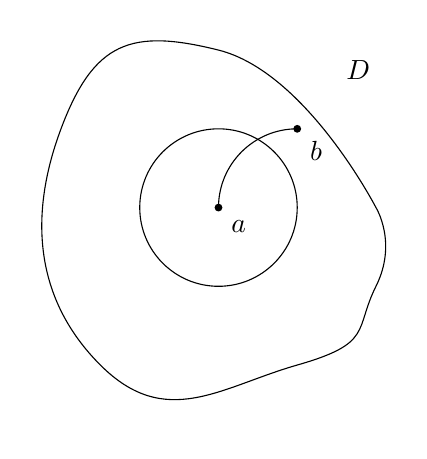
\begin{tikzpicture}
            \draw (0,0) circle (1);
            \draw [-] plot [smooth, tension=1] coordinates {(2,0) (0,2) (-2,1) (-1.5,-2) (1,-2) (2,-1) (2,0)};
            \node[fill,circle,inner sep=1pt,label=below right:$a$] at (0,0) {};
            \node[fill,circle,inner sep=1pt,label=below right:$b$] at (1,1) {};
            \draw[-] (0,0) arc (180:90:1);
            \node[above right] at (1.5, 1.5) {$D$};
        \end{tikzpicture}
    };

    \node(c) at (10, -5) {$\mathbb C$};
    \draw[->] (a) -- (b);
    \node[above] at (5,0) {$\Phi^{1-1}$};
    \draw[->] (a) -- (c);
    \node[below] at (6,-3.5) {$P\cdot \Phi$};
    \draw[->] (b) -- (c);
    \node[right] at (10, -3.5) {$P(z)$};
\end{tikzpicture}
\end{document}